This is the section in which I will briefly outline R-NET, the other model that I used for Reading Comprehension. In this case I also used DeepPavlov's pretrained model. R-NET is trained on SQuAD, dataset described in the relative BERT's section.

R-NET is an end-to-end neural networks model for reading comprehension \cite{rnet}. It performs this task similarly to the way in which we do it: reading the passage (i.e. the patient's sentence) multiple times. Basically, R-NET tries to improve the passage representation step after step, which are in total three:
\begin{enumerate}
  \item \textit{Question and Passage GRU Layer}. In this layer tokens are converted in GloVe embeddings, and for out-of-vocabulary tokens a character embedding is computed. Unfortunately, these vectors are not contextual: it is for this reason that these embeddings are then fed to a BiRNN (composed by Gated Recurrent Units) in order to ameliorate these representations.
  \item \textit{Question and Passage Matching Layer}. The aim of this layer is to encode the question terms into the passage embeddings of the previous layer. In other words, this permits to the network, given a token in the passage, to focus only on the relevant tokens in the question and tune the passage embeddings to be more similar to the relevant question embeddings. This is done using \textit{Attention}.
  
An example may be clearer \cite{understandingrnet}. Assuming we are at the highlighted word in the passage:

\begin{displayquote}
She had a talent for \textbf{making} home craft tools, mechanical appliances, and the ability to memorize Serbian epic poems.
\end{displayquote}

Given the highlighted token ``making'', Attention over the question tokens will highlight the word in bold:

\begin{displayquote}
What were Tesla's mother's special \textbf{abilities}?
\end{displayquote}

In this case, ``making'' embedding is adjusted in order to get it closer to ``abilities'' embedding. Doing so, R-NET encodes the question in the passage.

  \item \textit{Passage Self-Matching Layer}. Consider the following passage:
  
  \begin{displayquote}
  Tesla’s mother, Đuka Tesla (née Mandić), whose father was also an Orthodox priest, had a talent for making home craft tools, mechanical appliances, and the \textbf{ability} to memorize Serbian epic poems. Đuka had never received a formal education. Nikola credited his eidetic memory and creative \textbf{abilities} to his mother’s genetics and influence.
  \end{displayquote}
  
  It is clear that the term``ability'' refers to the mother of Tesla, while ``abilities'' refers to Nikola Tesla. The objective of this step is to capture the difference between terms like those, that, without context, are identical.
  
  Another difficulty resides in \textit{long-term dependencies}: ``ability'', for example, is far away from the subject to which the term is referred (Tesla's mother). However, GRU (creator, 2014) were developed for addressing the problem of the \textit{vanishing gradients}, which is the reason why vanilla RNNs have troubles with long-term dependencies.
  
  To resolve the former problem, R-NET introduces \textit{Self-Matched Attention}. While with Attention we use a passage term to weight a set of vectors (the question terms), with Self-Matched Attention R-NET use the current passage term to weigh tokens from the passage itself. This helps to differentiate the current term with similar-meaning terms in the rest of the passage.
\end{enumerate}

Having read and analyzed for three times the passage in the light of the question, the last layer is aimed to output the start and the end of the answer within the passage.

\begin{figure}[t]
% https://slideplayer.com/slide/12351679/
\centering
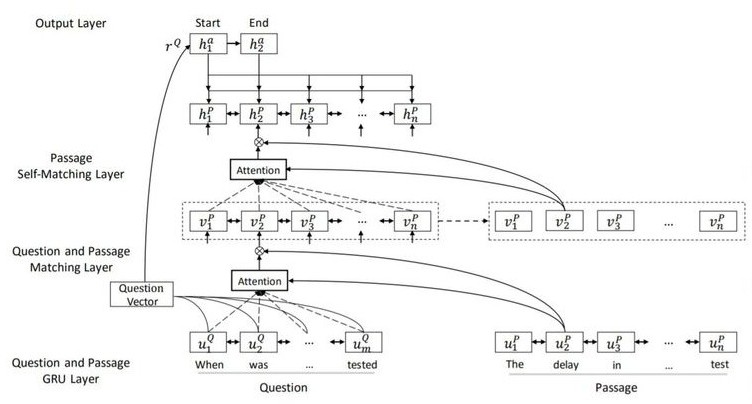
\includegraphics[width=15cm]{rnet}
\caption{A simplified overview of R-NET \cite{imagernetoverview}}
\medskip
\end{figure}
